\chapter{Sample chapter}\label{chap:sample}

\section{Math}

\subsection{Symbols}

\begin{itemize}
  \item Caligraphic letters: $\mathcal{A}$ 
  \item Mathbb letters: $\mathbb{A}$
  \item Mathfrak letters: $\mathfrak{A}$
  \item Math Sans serif letters: $\mathsf{A}$
  \item Math bold letters: $\mathbf{A}$
  \item Math bold upright greek letters: $\mathbf{\alpha}$ (Not displaying! Use the following one.)
  \item Math bold upright greek letters: $\symbfup{\alpha}$
  \item Math bold italic greel letters: $\bm{\alpha}$
  \item Math bold italic greek letters: $\mathbi{A}$
\end{itemize}

Avoid using \lstinline|bm| package as it conflicts with \lstinline|unicode-math| and it is outdated for \hologo{XeLaTeX}.
You can alias some math commands by \lstinline|\newcommand| or \lstinline|\renewcommand| anyway.

\subsection{Equations}

\begin{equation}
  E^2 = m^2 + p^2\label{eq:mass-energy}
\end{equation}

You can use \lstinline|\cref{}| to automatically setup the cross reference name; instead, you can always use \lstinline|\ref{}| to customize the appearence of the cross reference.

\cref{eq:mass-energy} or Equation (\ref{eq:mass-energy}) gives the mass-energy relationship.

\subsection{Theorem}

\begin{definition}
  LCL is orange juice.
\end{definition}

\begin{proof}
  They are both orange.
\end{proof}

Available theorem environments are listed below:

algorithm, assumption, axiom, conclusion, condition, corollary, definition, example, lemma, proof, property, proposition, remark, theorem.


\section{Figure}

\begin{figure}[H]
  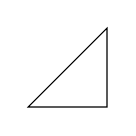
\begin{tikzpicture}
    \draw (0,0) -- (1, 0) -- (1, 1) -- cycle;
  \end{tikzpicture}
  \caption{An example tikz picture with long caption and breakline\\\blindtext}
  \label{fig:tikz example}
\end{figure}

An example image is shown in \cref{fig:tikz example} or Figure (\ref{fig:tikz example}).

\section{Table}

\begin{table}[H]
  \caption{Test result on different platforms}
  \label{tab:environment}
  \centering
  \begin{tabular}{lll}
    \toprule
    OS & TeX & Test \\
    \midrule
    Overleaf                 & \hologo{TeX}\,Live 2021/2/3    & Pass \\
    Arch Linux (2023.11)     & \hologo{TeX}\,Live           & Pass \\
    Windows 10/11            & \hologo{TeX}\,Live 2021      & Pass \\
    macOS 10.15              & \hologo{TeX}\,Live 2021      & Pass \\
    Windows 10               & \hologo{TeX}\,Live 2020      & \color{red}{\verb|ltxhook| problem} \\
    Ubuntu 20.04             & \hologo{TeX}\,Live 2021      & Pass \\
    Termux                   & \hologo{TeX}\,Live 2021      & Pass \\
    Windows 11               & \hologo{MiKTeX} 4.9          & Pass \\
    Windows 10               & \hologo{MiKTeX} 4.4          & Pass \\
    Ubuntu 20.04             & \hologo{MiKTeX} 4.2.1        & \color{red}{Failed} \\
    \bottomrule
  \end{tabular}
\end{table}


\section{Code}

\subsection{Inline code}
Use \lstinline$\lstinline|<code>|$ to print code snippets. The \lstinline$||$ marks delimit
the code and can be replaced by any character not in the code;
\textit{e.g.}   \lstinline|\lstinline$<code>$| gives the same result.

\subsection{Code environment}
The code to draw the \cref{fig:tikz example} is listed below:
\begin{lstlisting}[caption={\hologo{LaTeX} code for inserting a figure}]
\begin{figure}[htb]
  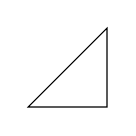
\begin{tikzpicture}
    \draw (0,0) -- (1, 0) -- (1, 1) -- cycle;
  \end{tikzpicture}
  \caption{An example picture with long caption: \blindtext\\\blindtext}
  \label{fig:tikz example} % this is a comment
\end{figure}
\end{lstlisting}

\section{Manage citations}
\label{chap:bibliography}

Use \lstinline|biber| as \hologo{BibTeX} backend.

\subsection{Add and manage}

Entries are stored in \lstinline|mythesis.bib|. For other sources, modify following commands in \lstinline|mythesis.tex|:
\begin{lstlisting}[language=TeX]
\addbibresource{mythesis.bib}
\end{lstlisting}

\subsection{Citation style}

As described in the sample page from ECE department, the style is set to \lstinline|ieee|. You can modify the style in the \lstinline|hkustthesis.cls| file as you wish.
